\documentclass[10pt,ignorenonframetext,,aspectratio=149]{beamer}
\usefonttheme{serif} % use mainfont rather than sansfont for slide text
\setbeamertemplate{caption}[numbered]
\setbeamertemplate{caption label separator}{: }
\setbeamercolor{caption name}{fg=normal text.fg}
\usepackage{lmodern}
\usepackage{amssymb,amsmath}
\usepackage{ifxetex,ifluatex}
\usepackage{fixltx2e} % provides \textsubscript
\ifnum 0\ifxetex 1\fi\ifluatex 1\fi=0 % if pdftex
  \usepackage[T1]{fontenc}
  \usepackage[utf8]{inputenc}
\else % if luatex or xelatex
  \ifxetex
    \usepackage{mathspec}
  \else
    \usepackage{fontspec}
  \fi
  \defaultfontfeatures{Ligatures=TeX,Scale=MatchLowercase}
  \newcommand{\euro}{€}
    \setmainfont[]{Open Sans}
\fi
% use upquote if available, for straight quotes in verbatim environments
\IfFileExists{upquote.sty}{\usepackage{upquote}}{}
% use microtype if available
\IfFileExists{microtype.sty}{%
\usepackage{microtype}
\UseMicrotypeSet[protrusion]{basicmath} % disable protrusion for tt fonts
}{}
\usepackage{graphicx,grffile}
\makeatletter
\def\maxwidth{\ifdim\Gin@nat@width>\linewidth\linewidth\else\Gin@nat@width\fi}
\def\maxheight{\ifdim\Gin@nat@height>\textheight0.8\textheight\else\Gin@nat@height\fi}
\makeatother
% Scale images if necessary, so that they will not overflow the page
% margins by default, and it is still possible to overwrite the defaults
% using explicit options in \includegraphics[width, height, ...]{}
\setkeys{Gin}{width=\maxwidth,height=\maxheight,keepaspectratio}

% Comment these out if you don't want a slide with just the
% part/section/subsection/subsubsection title:
\AtBeginPart{
  \let\insertpartnumber\relax
  \let\partname\relax
  \frame{\partpage}
}
\AtBeginSection{
  \let\insertsectionnumber\relax
  \let\sectionname\relax
  \frame{\sectionpage}
}
\AtBeginSubsection{
  \let\insertsubsectionnumber\relax
  \let\subsectionname\relax
  \frame{\subsectionpage}
}

\setlength{\emergencystretch}{3em}  % prevent overfull lines
\providecommand{\tightlist}{%
  \setlength{\itemsep}{0pt}\setlength{\parskip}{0pt}}
\setcounter{secnumdepth}{0}

\title{Hypothesis Tests and Model Selection}
\author{Henrique Veras}
\date{}

%% Here's everything I added.
%%--------------------------

\usepackage{graphicx}
\usepackage{rotating}
%\setbeamertemplate{caption}[numbered]
\usepackage{hyperref}
\usepackage{caption}
\usepackage[normalem]{ulem}
%\mode<presentation>
\usepackage{wasysym}
%\usepackage{amsmath}


% Get rid of navigation symbols.
%-------------------------------
\setbeamertemplate{navigation symbols}{}

% Optional institute tags and titlegraphic.
% Do feel free to change the titlegraphic if you don't want it as a Markdown field.
%----------------------------------------------------------------------------------
\institute{PIMES/UFPE}

% \titlegraphic{\includegraphics[width=0.3\paperwidth]{\string~/Dropbox/teaching/clemson-academic.png}} % <-- if you want to know what this looks like without it as a Markdown field. 
% -----------------------------------------------------------------------------------------------------


% Some additional title page adjustments.
%----------------------------------------
\setbeamertemplate{title page}[empty]
%\date{}
\setbeamerfont{subtitle}{size=\small}

\setbeamercovered{transparent}

% Some optional colors. Change or add as you see fit.
%---------------------------------------------------
\definecolor{clemsonpurple}{HTML}{522D80}
 \definecolor{clemsonorange}{HTML}{F66733}
\definecolor{uiucblue}{HTML}{003C7D}
\definecolor{uiucorange}{HTML}{F47F24}


% Some optional color adjustments to Beamer. Change as you see fit.
%------------------------------------------------------------------
\setbeamercolor{frametitle}{fg=clemsonpurple,bg=white}
\setbeamercolor{title}{fg=clemsonpurple,bg=white}
\setbeamercolor{local structure}{fg=clemsonpurple}
\setbeamercolor{section in toc}{fg=clemsonpurple,bg=white}
% \setbeamercolor{subsection in toc}{fg=clemsonorange,bg=white}
\setbeamercolor{footline}{fg=clemsonpurple!50, bg=white}
\setbeamercolor{block title}{fg=clemsonorange,bg=white}


\let\Tiny=\tiny


% Sections and subsections should not get their own damn slide.
%--------------------------------------------------------------
\AtBeginPart{}
\AtBeginSection{}
\AtBeginSubsection{}
\AtBeginSubsubsection{}

% Suppress some of Markdown's weird default vertical spacing.
%------------------------------------------------------------
\setlength{\emergencystretch}{0em}  % prevent overfull lines
\setlength{\parskip}{0pt}


% Allow for those simple two-tone footlines I like. 
% Edit the colors as you see fit.
%--------------------------------------------------
\defbeamertemplate*{footline}{my footline}{%
    \ifnum\insertpagenumber=1
    \hbox{%
        \begin{beamercolorbox}[wd=\paperwidth,ht=.8ex,dp=1ex,center]{}%
      % empty environment to raise height
        \end{beamercolorbox}%
    }%
    \vskip0pt%
    \else%
        \Tiny{%
            \hfill%
		\vspace*{1pt}%
            \insertframenumber/\inserttotalframenumber \hspace*{0.1cm}%
            \newline%
            \color{clemsonpurple}{\rule{\paperwidth}{0.4mm}}\newline%
            \color{clemsonorange}{\rule{\paperwidth}{.4mm}}%
        }%
    \fi%
}

% Various cosmetic things, though I must confess I forget what exactly these do and why I included them.
%-------------------------------------------------------------------------------------------------------
\setbeamercolor{structure}{fg=blue}
\setbeamercolor{local structure}{parent=structure}
\setbeamercolor{item projected}{parent=item,use=item,fg=clemsonpurple,bg=white}
\setbeamercolor{enumerate item}{parent=item}

% Adjust some item elements. More cosmetic things.
%-------------------------------------------------
\setbeamertemplate{itemize item}{\color{clemsonpurple}$\bullet$}
\setbeamertemplate{itemize subitem}{\color{clemsonpurple}\scriptsize{$\bullet$}}
\setbeamertemplate{itemize/enumerate body end}{\vspace{.6\baselineskip}} % So I'm less inclined to use \medskip and \bigskip in Markdown.

% Automatically center images
% ---------------------------
% Note: this is for ![](image.png) images
% Use "fig.align = "center" for R chunks

\usepackage{etoolbox}

\AtBeginDocument{%
  \letcs\oig{@orig\string\includegraphics}%
  \renewcommand<>\includegraphics[2][]{%
    \only#3{%
      {\centering\oig[{#1}]{#2}\par}%
    }%
  }%
}

% I think I've moved to xelatex now. Here's some stuff for that.
% --------------------------------------------------------------
% I could customize/generalize this more but the truth is it works for my circumstances.

\ifxetex
\setbeamerfont{title}{family=\fontspec{Titillium Web}}
\setbeamerfont{frametitle}{family=\fontspec{Titillium Web}}
\usepackage[font=small,skip=0pt]{caption}
 \else
 \fi

% Okay, and begin the actual document...

\begin{document}
\frame{\titlepage}

\hypertarget{econometrics}{%
\section{Econometrics}\label{econometrics}}

\hypertarget{intro}{%
\subsection{Intro}\label{intro}}

\begin{frame}{Intro}
Purposes of linear regression models:

\begin{enumerate}
\tightlist
\item
  Estimation
\item
  Prediction
\item
  Hypothesis testing
\end{enumerate}
\end{frame}

\hypertarget{hypothesis-testing-methodology}{%
\subsection{Hypothesis Testing
Methodology}\label{hypothesis-testing-methodology}}

\begin{frame}{Hypothesis Testing Methodology}
\protect\hypertarget{hypothesis-testing-methodology-1}{}
We start by providing a general framework for conducting hypothesis
testing.

\vfill

The general approach to testing a hypothesis is to formulate a
statistical model that contains the hypothesis as a restriction on the
model's parameters.

\vfill

Consider a model of investment:

\[\ln I_t = \beta_1 + \beta_2 i_t + \beta_3 \Delta p_t + \beta_4 \ln Y_t + \beta_5 t + \varepsilon_t\]

\vfill

This theory states that investment is a function of the \emph{nominal}
interest rate, inflation rate, income, and factors that evolve together
over time.

\vfill

Let's call this model 1.

\vfill
\end{frame}

\begin{frame}{Nested Models}
\protect\hypertarget{nested-models}{}
An alternative theory suggests that investors care about \emph{real}
interest rates:

\[\ln I_t = \beta_1 + \beta_2 (i_t - \Delta p_t) + \beta_3 \Delta p_t + \beta_4 \ln Y_t + \beta_5 t + \varepsilon_t\]

\vfill

This theory, however, does not have a testable implication for our
model.

\vfill

If, instead, we impose a \textbf{restriction} on model 1 stating that
``investors care \emph{only} about real interest rates, the equation
would become model 2 below:

\[\ln I_t = \beta_1 + \beta_2 (i_t - \Delta p_t )+ \beta_4 \ln Y_t + \beta_5 t + \varepsilon_t\]

\vfill

In this case, model 2 is the same as model 1 with the added restriction
that \(\beta_2 = -\beta_3\) or \(\beta_2 + \beta_3 = 0\).

\vfill
\end{frame}

\begin{frame}{Nested Models}
\protect\hypertarget{nested-models-1}{}
We, then, say that models 1 and 2 are nested.

\vfill

The parameter space of the \emph{restricted} model (model 2) is smaller
than the parameter space of the \emph{unrestricted} model (model 1).

\vfill
\end{frame}

\begin{frame}{Size, Power, and Consistency of a Test}
\protect\hypertarget{size-power-and-consistency-of-a-test}{}
Prior to conducting a hypothesis testing, such as whether investors care
only about real interest rates, we define a rejection (and acceptance)
region, which indicates whether we have gathered enough evidence against
a given theory.

\vfill

For instance, supoose we estimate

\[y=\beta_1 + \beta_2 x_1 + \beta_3 x_2 + \varepsilon\]

and impose a restriction \(\beta_3=0\). The classical hypothesis testing
procedure suggests to define two (mutually exclusive) hypotheses:

\[H_0: \beta_3 = 0\]

\[H_1: \beta_3 \neq 0\]
\end{frame}

\begin{frame}{Size, Power, and Consistency of a Test}
\protect\hypertarget{size-power-and-consistency-of-a-test-1}{}
In performing a test, there are two ways in which we can incur in a
error (given the randomness of process):

\begin{enumerate}
\tightlist
\item
  Type I error: the null hypothesis is incorrectly rejected
\item
  Type II error: the null hypothesis is incorrectly retained.
\end{enumerate}

\vfill

The probability of a type I error is called the \textbf{size of the
test}.

\vfill

\(1-\text{Prob}(\text{Type II error})\) is called the \textbf{power of
the test}. This is the probability of correctly rejecting the null
hypothesis.

\vfill

A test procedure is \textbf{consistent} if its power goes to 1 as the
sample size goes to infinity. If a test is based on consistent
estimators, then the test itself is consistent.

\vfill
\end{frame}

\begin{frame}{Three Approaches to Testing Hypotheses}
\protect\hypertarget{three-approaches-to-testing-hypotheses}{}
\begin{enumerate}
\tightlist
\item
  Wald tests: based on estimation of the unrestricted model -- the test
  measures how close the estimated unrestricted model is to the
  hypothesis restrictions;
\end{enumerate}

\vfill

\begin{enumerate}
\setcounter{enumi}{1}
\tightlist
\item
  Fit based tests: comparing \(R^2\)s when we estimate the unrestricted
  model and when we incorporate the restriction.
\end{enumerate}

\vfill

\begin{enumerate}
\setcounter{enumi}{2}
\tightlist
\item
  Lagrange multiplier tests: based on correlation between variables from
  restriction and the residuals from the regression of restricted model.
\end{enumerate}

\vfill
\end{frame}

\begin{frame}{General Approach}
\protect\hypertarget{general-approach}{}
The general linear hypothesis is a set of \(J\) restrictions on the
linear regression model

\[y=\mathbf{X\beta}+\varepsilon\]

\vfill

The restrictions are

\[r_{11}\beta_1 + r_{12}\beta_2 + \cdots + r_{1K}\beta_K=q_1\]

\[r_{21}\beta_1 + r_{22}\beta_2 + \cdots + r_{2K}\beta_K=q_2\]

\[\vdots\]

\[r_{J1}\beta_1 + r_{J2}\beta_2 + \cdots + r_{JK}\beta_K=q_J\]

In matrix form:

\[\mathbf{R\beta}=\mathbf{q}\]

\vfill
\end{frame}

\begin{frame}{General Approach}
\protect\hypertarget{general-approach-1}{}
The hypotheses implied by the restrictions are written

\[H_0:\mathbf{R\beta}-\mathbf{q}=\mathbf{0}\]
\[H_1:\mathbf{R\beta}-\mathbf{q}\neq\mathbf{0}\]

Example: Assume you have a model with an intercept and 5 independent
variables:
\[y=\beta_0 + \beta_1 x_1 + \beta_2 x_2 + \beta_3 x_3 + \beta_4 x_4 + \beta_5 x_5 + \varepsilon\]

What are \(\mathbf{R}\) and \(\mathbf{q}\) in each case below?

\begin{enumerate}
\tightlist
\item
  \(\beta_3=0\)
\item
  \(\beta_2=\beta_3\)
\item
  \(\beta_1 + \beta_2 + \beta_3 = 1\)
\item
  \(\beta_1 = 0\), \(\beta_2 = 0\), \(\beta_3 = 0\)
\item
  \(\beta_1 + \beta_2 = 1\), \(\beta_3 + \beta_4 = 1\),
  \(\beta_5 + \beta_6 = 0\)
\item
  All coefficients in the model except the intercept are zero
\end{enumerate}

\vfill
\end{frame}

\begin{frame}{Some Information about \(\mathbf{R}\)}
\protect\hypertarget{some-information-about-mathbfr}{}
\begin{enumerate}
\tightlist
\item
  Full row rank (\(J\leq K\)) but we assume strict inequality
\item
  Rows must be linearly independent
\end{enumerate}
\end{frame}

\hypertarget{wald-tests-based-on-the-distance-measure}{%
\subsection{Wald Tests Based on the Distance
Measure}\label{wald-tests-based-on-the-distance-measure}}

\begin{frame}{Wald Tests Based on the Distance Measure}
Let's start by testing a hypothesis about a coefficient.

\vfill

Suppose we are interested in testing

\[H_0: \beta_k=\beta_k^0\]

The \textbf{Wald distance} of a coefficient estimate from a hypothesized
value is the distance measured in standard deviation units

\[W_k=\frac{b_k-\beta_k^0}{\sqrt{\sigma^2 S^{kk}}}\]

\(W_k\) follows a standard normal distribution if the null hypothesis is
true.

\vfill

Notice, however, that \(\sigma^2\) is unknown. We estimate it with
\(s^2\):

\[t_k=\frac{b_k-\beta_k^0}{\sqrt{s^2 S^{kk}}}\]
\end{frame}

\begin{frame}{Wald Tests Based on the Distance Measure}
\protect\hypertarget{wald-tests-based-on-the-distance-measure-1}{}
To construct a testing procedure, we define the rejection/acceptance
region by determining the \emph{confidence} with which we would like to
draw the conclusion.

\vfill

Using a 95\% confidence interval, we can say that

\[\text{Prob}[-t^*_{(1-\alpha/2),[n-K]}<t_k<t^*_{(1-\alpha/2),[n-K]}]\]

That is, if the null hypothesis is true, finding a value of \(t_k\)
outside this range is highly unlikely.

\vfill

It must be that the mean value \(\beta_k^0\) is not the one
hypothesized.

\vfill
\end{frame}

\begin{frame}{The F Statistic}
\protect\hypertarget{the-f-statistic}{}
We now consider testing a set of \(J\) linear restrictions

\[H_0:\mathbf{R\beta}-\mathbf{q}=\mathbf{0}\]
\[H_1:\mathbf{R\beta}-\mathbf{q}\neq\mathbf{0}\]

Given the LS estimator \(\mathbf{b}\), we are interested in the
\textbf{discrepancy vector} \(\mathbf{Rb}-\mathbf{q}=\mathbf{m}\).

\vfill

Our question is how far \(\mathbf{m}\) is from zero.

\vfill

Notice that \(\mathbf{m}\) is normally distributed, since it is a linear
combination of \(\mathbf{b}\), which is normally distributed.

\vfill
\end{frame}

\begin{frame}{The F Statistic}
\protect\hypertarget{the-f-statistic-1}{}
Let's find \(\mathbf{m}\)'s expected value and variance:

\[\begin{split} E[\mathbf{m}|\mathbf{X}] & =\mathbf{R}E[\mathbf{\beta}|\mathbf{X}]-\mathbf{q}=0 \\
Var[\mathbf{m}|\mathbf{X}] & =\mathbf{R}Var[\mathbf{\beta}|\mathbf{X}]\mathbf{R}'=\mathbf{R}\sigma^2(\mathbf{X'X})^{-1}\mathbf{R}'\end{split}\]

\vfill

The test statistic is given by

\[\begin{split}
W & =\mathbf{m}'Var[\mathbf{m}|\mathbf{X}]^{-1}\mathbf{m} \\
 & = (\mathbf{Rb}-\mathbf{q})'\sigma^2(\mathbf{X'X})^{-1}(\mathbf{Rb}-\mathbf{q}) \sim \chi^2[J]
\end{split}\]

\vfill

Thus, \(W\) follows a chi-squared distribution with \(J\) degrees of
freedom if the null hypothesis is correct.

\vfill
\end{frame}

\begin{frame}{The F Statistic}
\protect\hypertarget{the-f-statistic-2}{}
By estimating \(\sigma^2\) with \(s^2\) and dividing the result by
\(J\), we obtain a usable \(F\) statistic with \(J\) and \(n-K\) degrees
of freedom:

\[F[J,n-K|X]=\frac{(\mathbf{Rb}-\mathbf{q})'[\mathbf{R}s^2(\mathbf{X'X})^{-1}\mathbf{R}']^{-1}(\mathbf{Rb}-\mathbf{q})}{J}\]

\vfill

If we are interested in testing \emph{one} linear restriction of the
form

\[H_0: r_1 \beta_1 + r_2\beta_2 + \cdots + r_K\beta_K=\mathbf{r'\beta}=q,\]

the \(F\) statistic is

\[F[1,n-K]=\frac{\sum{ (r_j \beta_j-q)^2}}{\sum_j\sum_k(r_j r_kEst.Cov(b_j, b_k))}\]

\vfill

If the test if for \(\beta_j=q\), the \(F\) statistic is then

\[F(1, n-K)=\frac{(b_j-q)^2}{Est.Var(b_j)}\]

\vfill
\end{frame}

\begin{frame}{The F Statistic}
\protect\hypertarget{the-f-statistic-3}{}
Consider an alternative approach: find the sample estimate of
\(\mathbf{r'\beta}\)

\[r_1 b_1 + r_2b_2 + \cdots + r_Kb_K=\hat{\mathbf{q}}\]

The test statistic is \[t=\frac{\hat{q}-q}{se(\hat{q})}\]

where
\(Est.Var(\hat{q}|\mathbf{X})=\mathbf{r}'[s^2(\mathbf{X'X})^{-1}]\mathbf{r}\)

\vfill

It follows, therefore, that for testing a single restriction, the \(t\)
statistic is the square root of the \(F\) statistic that would be used
to test that hypothesis.

\vfill
\end{frame}

\hypertarget{tests-based-on-the-fit-of-the-regression}{%
\subsection{Tests based on the fit of the
regression}\label{tests-based-on-the-fit-of-the-regression}}

\begin{frame}{Tests based on the fit of the regression}
Another approach to hypothesis testing is asking whether choosing some
other value for the slopes of the regression leads to a significant loss
of fit.

\vfill

That is, we can compare \(R^2\)s from both unrestricted and restricted
models to test for a given hypothesis.

\vfill
\end{frame}

\begin{frame}{The Restricted LS Estimator}
\protect\hypertarget{the-restricted-ls-estimator}{}
If we explicitly impose the restrictions of the general linear
hypothesis, in the regression, we solve

\[Min_{\mathbf{b}_0}S(\mathbf{b}_0)=(\mathbf{y}-\mathbf{Xb}_0)'(\mathbf{y}-\mathbf{Xb}_0)\]

subject to \(\mathbf{R b}_0=\mathbf{q}\)

We can show that the solution to the restricted LS coefficient
\(\mathbf{b}_*\) is given by

\[\mathbf{b_*}=\mathbf{b}-(\mathbf{X'X})^{-1}\mathbf{R}'[\mathbf{R}(\mathbf{X'X})^{-1}\mathbf{R}']^{-1}(\mathbf{Rb}-\mathbf{q})\]

\[\lambda_*=[\mathbf{R}(\mathbf{X'X})^{-1}\mathbf{R}']^{-1}(\mathbf{Rb}-\mathbf{q})\]

\vfill
\end{frame}

\begin{frame}{The Restricted LS Estimator}
\protect\hypertarget{the-restricted-ls-estimator-1}{}
Moreover, Greene and Seaks (1991) show that \(Var[\mathbf{b}_*|X]\) is
simply \(\sigma^2\) times the upper left block of \(\mathbf{A}^{-1}\):

\[(\mathbf{X'X})^{-1}(\mathbf{I}-\mathbf{R}'[\mathbf{R}(\mathbf{X'X})^{-1}\mathbf{R}']^{-1}\mathbf{R}(\mathbf{X'X})^{-1}\]

\vfill

Thus,

\[\begin{split} Var[\mathbf{b}_*|X] & = \sigma^2(\mathbf{X'X})^{-1}-\sigma^2(\mathbf{X'X})^{-1}\mathbf{R}'[\mathbf{R}(\mathbf{X'X})^{-1}\mathbf{R}']^{-1}\mathbf{R}(\mathbf{X'X})^{-1}\\
 & = Var[\mathbf{b}|X] - \text{a nonnegative matrix}\end{split}\]

\vfill

One intuition for the difference
\(Var[\mathbf{b}|X]<Var[\mathbf{b}_*|X]\) is the value of the new
information brought by the restrictions.

\vfill
\end{frame}

\begin{frame}{The Loss of Fit from Restricted LS}
\protect\hypertarget{the-loss-of-fit-from-restricted-ls}{}
Let's first consider the case of a restriction on a single coefficient.

\vfill

Recall from Theorem 3.6, which shows the change in the \(R^2\) following
the introduction of a variable \(z\) to the model:

\[R^2_{Xz}=R^2_X+(1-R^2_X)r^{*2}_{yz}\]

\vfill

A convenient result is that

\[r^{*2}_{yz}=\frac{t_z^2}{t_z^2+(n-K)},\] where \(t_z^2\) is the square
of the t ratio for testing the hypothesis that the coefficient on z is
zero in the multiple regression of \(\mathbf{y}\) on \(\mathbf{X}\) and
\(\mathbf{z}\).

\vfill
\end{frame}

\begin{frame}{The Loss of Fit from Restricted LS}
\protect\hypertarget{the-loss-of-fit-from-restricted-ls-1}{}
Substituting one equation into the other, we obtain

\[t_z^2=\frac{(R^2_{Xz}-R^2_{X})/1}{(1-R^2_{Xz})/(n-K)}\]

\vfill

As we saw before, \(t^2(n-K)=F[1,n-K]\). Then, the statistic above
follows an F distribution with 1 and \(n-K\) d.f.

\vfill
\end{frame}

\begin{frame}{The Loss of Fit from Restricted LS}
\protect\hypertarget{the-loss-of-fit-from-restricted-ls-2}{}
Let's now find a general representation for the above procedure.

\vfill

First, notice that the fit of the restricted LS cannot be better than
the restricted solution:

\vfill

Let \(\mathbf{e}_*=\mathbf{y}-\mathbf{Xb}_*\). Adding and subtracting
\(\mathbf{Xb}\), we can write

\[\mathbf{e}_*=\mathbf{e}-\mathbf{X}(\mathbf{b}_*-\mathbf{b})\]

The new sum of squared deviations is

\[\mathbf{e}_*'\mathbf{e}_*=\mathbf{e}'\mathbf{e}+(\mathbf{b}_*-\mathbf{b})'\mathbf{X'X}(\mathbf{b}_*-\mathbf{b})\geq \mathbf{e}'\mathbf{e}\]

\vfill
\end{frame}

\begin{frame}{The Loss of Fit from Restricted LS}
\protect\hypertarget{the-loss-of-fit-from-restricted-ls-3}{}
We define the loss of fit as the difference in the sum of squared
residuals from the restricted model and the sum of squared residuals
from the restricted model:

\[\mathbf{e}_*'\mathbf{e}_*-\mathbf{e}'\mathbf{e}=(\mathbf{b}_*-\mathbf{b})'\mathbf{X'X}(\mathbf{b}_*-\mathbf{b})\]

\vfill

Recall:

\[\mathbf{b_*}-\mathbf{b}=(\mathbf{X'X})^{-1}\mathbf{R}'[\mathbf{R}(\mathbf{X'X})^{-1}\mathbf{R}']^{-1}(\mathbf{Rb}-\mathbf{q})\]

Thus, substituting this in the previous expression, we find

\[\mathbf{e}_*'\mathbf{e}_*=(\mathbf{Rb}-\mathbf{q})'[\mathbf{R}(\mathbf{X'X})^{-1}\mathbf{R}']^{-1}(\mathbf{Rb}-\mathbf{q})\]

\vfill
\end{frame}

\begin{frame}{The Loss of Fit from Restricted LS}
\protect\hypertarget{the-loss-of-fit-from-restricted-ls-4}{}
This expression appears in the numerator of the F statistic. Inserting
the remaining parts:

\[F[J,n-K]=\frac{(\mathbf{e}_*'\mathbf{e}_*-\mathbf{e}'\mathbf{e})/J}{\mathbf{e}'\mathbf{e}/(n-K)}\]

Dividing both numerator and denominator by \(\sum_i{(y_i-\bar{y})^2}\),
we have

\[F[J,n-K]=\frac{(R^2-R^2_*)/J}{(1-R^2)/(n-K)}\]

\vfill

This means that large values of F give evidence against the validity of
the hypothesis.

\vfill
\end{frame}

\begin{frame}{Testing the Significance of the Regression}
\protect\hypertarget{testing-the-significance-of-the-regression}{}
A relevant question is whether the regression equation as a whole is
significant (that's question 6 from our previous example).

\vfill

This is a special case with \(R^2_*=0\), so that the F statistic become

\[F[K-1,n-K]=\frac{R^2/(K-1)}{(1-R^2)/(n-K)}\]
\end{frame}

\hypertarget{lagrange-multiplier-tests}{%
\subsection{Lagrange Multiplier Tests}\label{lagrange-multiplier-tests}}

\begin{frame}{Lagrange Multiplier Tests}
Recall the solution for the Lagrange multiplier:

\[\mathbf{\lambda}_*=[\mathbf{R}(\mathbf{X'X})^{-1}\mathbf{R}']^{-1}(\mathbf{Rb}-\mathbf{q})\]

\vfill

Lagrange multiplier tests rely on the idea that testing whether
\(\lambda_*=0\) should be equivalent to testing
\(\mathbf{R\beta}-\mathbf{q}=\mathbf{0}\) (why?)

\vfill

The chi-square test statistic is computed as

\[W_{LM}=(\mathbf{Rb}-\mathbf{q})'[\mathbf{R}\sigma^2(\mathbf{X'X})^{-1}\mathbf{R}']^{-1}(\mathbf{Rb}-\mathbf{q})\]

A feasible version of this test statistic is obtained by using \(s^2\)
(from the restricted model) in place of the unknown \(\sigma^2\).

\vfill
\end{frame}

\hypertarget{large-sample-tests}{%
\subsection{Large Sample Tests}\label{large-sample-tests}}

\begin{frame}{Large Sample Tests}
Without the normality assumption, the exact distributions of the test
statistics that we calculated before depend on the data and the
parameters.

\vfill

They are no longer \(t\), \(F\), and chi-squared.

\vfill

Recall:

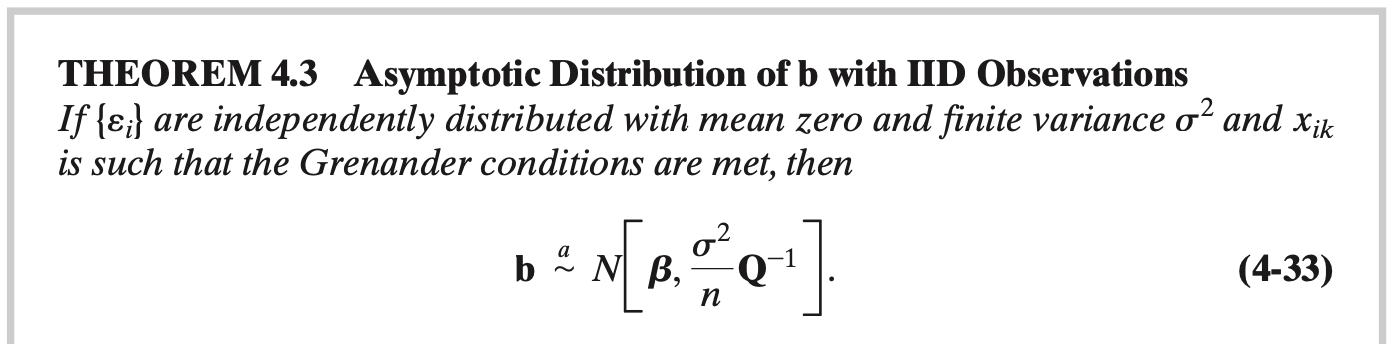
\includegraphics{/Users/henriquefonseca/Desktop/temp/Rmarkdown-practice/henriqueveras.github.io/files/Econometrics/Lecture Notes/3/theorem_4.3.png}

\vfill

and \(\text{plim } s^2=\sigma^2\)
\end{frame}

\begin{frame}{Large Sample Tests}
\protect\hypertarget{large-sample-tests-1}{}
The test statistic for testing some hypothesis about a given \(\beta_k\)
is

\[t_k=\frac{\sqrt{n}(b_k-\beta_k^0)}{\sqrt{s^2(\mathbf{X'X}/n)^{-1}_{kk}}}\]

\vfill

Notice that this is the same as before, as \(\sqrt{n}\) cancels out.

\vfill

Without normality, the exact distribution of this statistic is unknown.

\vfill

The denominator of \(t_k\) converges to
\(\sqrt{\sigma^2\mathbf{Q}_{kk}^{-1}}\), where
\(\mathbf{Q}=\text{plim }\frac{\mathbf{X'X}}{n}\).

\vfill
\end{frame}

\begin{frame}{Large Sample Tests}
\protect\hypertarget{large-sample-tests-2}{}
Therefore,

\[\tau_k=\frac{\sqrt{n}(b_k-\beta_k^0)}{\sqrt{\sigma^2\mathbf{Q}^{-1}_{kk}}}\]

\vfill

Thus, \(\tau_k\) follows (asymptotically) a standard normal distribution
under the null hypothesis.

\vfill
\end{frame}

\begin{frame}{Large Sample Tests}
\protect\hypertarget{large-sample-tests-3}{}
As for the \(F\) test, we can multiply numerator and denominator by
\(\sigma^2\) and rearreange it to find

\[F=\frac{(\mathbf{Rb}-\mathbf{q})'[\mathbf{R}\sigma^2(\mathbf{X'X})^{-1}\mathbf{R}']^{-1}(\mathbf{Rb}-\mathbf{q})}{J(s^2/\sigma^2)}\]

\vfill

If \(F\) has a limiting distribution, then it is the same as the
limiting distribution of

\[\begin{split} W^* & = \frac{1}{J}(\mathbf{Rb}-\mathbf{q})'[\mathbf{R}(\sigma^2/n)\mathbf{Q}^{-1}\mathbf{R}']^{-1}(\mathbf{Rb}-\mathbf{q})\\
 & = \frac{1}{J}(\mathbf{Rb}-\mathbf{q})'[Asy.Var(\mathbf{Rb}-\mathbf{q})]^{-1}(\mathbf{Rb}-\mathbf{q})\end{split}\]

\vfill

Recall that
\(Var[\mathbf{Rb}-\mathbf{q|\mathbf{X}}]=\mathbf{R}\sigma^2(\mathbf{X'X})^{-1}\mathbf{R}'\).

\vfill

This expression is \(1/J\) multiplied by a Wald statistic, based on the
asymptotic distribution.

\vfill
\end{frame}

\begin{frame}{Limiting Distribution of the Wald Statistic}
\protect\hypertarget{limiting-distribution-of-the-wald-statistic}{}
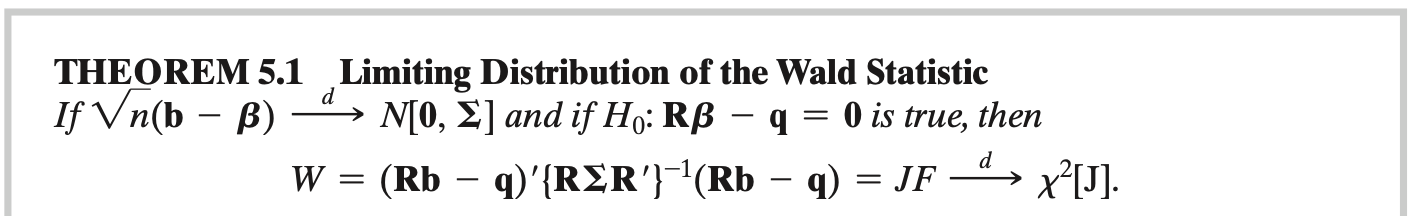
\includegraphics{/Users/henriquefonseca/Desktop/temp/Rmarkdown-practice/henriqueveras.github.io/files/Econometrics/Lecture Notes/5/theorem_5.1.png}
\end{frame}

\hypertarget{testing-nonlinear-restrictions}{%
\subsection{Testing Nonlinear
Restrictions}\label{testing-nonlinear-restrictions}}

\begin{frame}{Testing Nonlinear Restrictions}
Suppose now we are interested in testing a hypothesis that involves a
nonlinear function of the regression coefficients:

\[H_0: c(\mathbf{\beta})=\mathbf{q}\]

The test statistic is

\[z=\frac{c(\hat{\mathbf{\beta}})-q}{\text{estimated st. error}}\]

\vfill

The numerator can be easily obtained. To find the estimated variance,
however, we rely on a Taylor series approximation around the true
parameter \(\beta\):

\[c(\hat{\beta})\approx c(\beta)+\left(\frac{\partial c(\beta)}{\partial \beta}\right)'(\hat{\beta}-\beta)\]

Thus,

\[Var[c(\hat{\beta})]\approx\left(\frac{\partial c(\beta)}{\partial \beta}\right)'Asy.Var[\hat{\beta}]\left(\frac{\partial c(\beta)}{\partial \beta}\right)\].

\vfill
\end{frame}

\begin{frame}{Testing Nonlinear Restrictions}
\protect\hypertarget{testing-nonlinear-restrictions-1}{}
We use \(\mathbf{b}\) as an estimator of \(\beta\) and estimate
\(c(\mathbf{\beta})\) with \(c(\mathbf{b})\).

\vfill

According to the Slutsky theorem, if \(\text{plim }b=\beta\), then
\(\text{plim }c(b)=c(\beta)\).
\end{frame}

\hypertarget{choosing-between-nonnested-models}{%
\subsection{Choosing Between Nonnested
Models}\label{choosing-between-nonnested-models}}

\begin{frame}{Choosing Between Nonnested Models}
Suppose that, for example, we are now interested in testing whether a
linear or a log-linear model is appropriate, or determining which of two
possible sets of regressors is more appropriate.

\vfill

We are interested in comparing two competing linear models:

\[H_0: \mathbf{y}=\mathbf{X\beta}+\mathbf{\varepsilon}_1\]

\[H_1: \mathbf{y}=\mathbf{Z\gamma}+\mathbf{\varepsilon}_2\]

Notice how the models are nonnested. In this case, how do we perform a
test? Is the usual size of the test in this case useful?

\vfill
\end{frame}

\begin{frame}{An Encompassing Model}
\protect\hypertarget{an-encompassing-model}{}
We say Model 0 \emph{encompasses} Model 1 if the features of Model 1 can
be explained by model 0, but the reverse is not true.

\vfill

Let \(\bar{\mathbf{X}}\) denote the set of variables in \(\mathbf{X}\)
that are not in \(\mathbf{Z}\) and define \(\bar{\mathbf{Z}}\) likewise
with respect to \(\mathbf{X}\).

\vfill

Moreover, let \(\mathbf{W}\) be the set of variables that the models
have in common.

\vfill

Then, \(H_0\) and \(H_1\) can be combined in a supermodel:

\[\mathbf{y}= \bar{\mathbf{X}}\bar{\mathbf{\beta}} + \bar{\mathbf{Z}}\bar{\mathbf{\gamma}}+ \mathbf{W}\mathbf{\delta}+ \mathbf{\varepsilon}\]

\vfill
\end{frame}

\begin{frame}{An Encompassing Model}
\protect\hypertarget{an-encompassing-model-1}{}
\(H_0\) can be rejected if it is found that \(\bar{\mathbf{\beta}}=0\)
and \(H_1\) likewise for \(\bar{\mathbf{\gamma}}=0\).

\vfill

This test can be performed applying a conventional \(F\) test.

\vfill

Problems with this approach:

\begin{enumerate}
\tightlist
\item
  We cannot test whether \(\mathbf{\beta}\) or \(\mathbf{\gamma}\) are
  zero. why?
\item
  This compound model can have an extremely large set of regressors.
\end{enumerate}

\vfill
\end{frame}

\begin{frame}{An Alternative Approach}
\protect\hypertarget{an-alternative-approach}{}
Suppose \(H_0\) is correct. Then, we can estimate \(\mathbf{\gamma}\) by
regressing \(\mathbf{y}\) on \(\mathbf{Z}\), which yields an estimator
vector, say, \(\mathbf{c}\).

\vfill

If we regress \(\mathbf{X\beta}\) on \(\mathbf{Z}\), we should find the
exact same coefficients, say \(\mathbf{c}_0\) (assuming
\(\mathbf{\varepsilon}\)'s are random noises). Why?

\vfill

A test for the proposition that Model 0 encompasses Model 1 is whether
\(E[\mathbf{c}-\mathbf{c}_0]=0\)

\vfill
\end{frame}

\begin{frame}{Comprehensive Approach -- The J Test}
\protect\hypertarget{comprehensive-approach-the-j-test}{}
The \(J\) test, proposed by Davidson and MacKinnon (1981) suggests an
alternative:

\[\mathbf{y}=(1-\lambda)\mathbf{X\beta}+\lambda\mathbf{Z\gamma}+\mathbf{\varepsilon}\]

\vfill

A test of \(\lambda=0\) would be against \(H_1\). However, this cannot
be separately estimated.

\vfill

The \(J\) test consists of estimating \(\mathbf{\gamma}\) by LS
regression of \(\mathbf{y}\) on \(\mathbf{Z}\) followed by a LS
regression of \(\mathbf{y}\) on \(\mathbf{X}\) and \(\mathbf{Z\gamma}\)

\vfill

Asymptotically, \(\hat{\lambda}/se(\hat{\lambda})\) is distributed as
standard normal.
\end{frame}

\hypertarget{a-specification-test}{%
\subsection{A Specification Test}\label{a-specification-test}}

\begin{frame}{A Specification Test}
Finally, the idea now is to consider a particular null model and
alternatives that are not explicitly given in the form of restrictions
on the regression equation.

\vfill

Ramsey's (1967) RESET test:

\[\begin{split} H_0: \mathbf{y}= & \mathbf{X\beta}+\mathbf{\varepsilon} \\
H_1: \mathbf{y}= & \mathbf{X\beta}+ \text{higher order powers of } x_k \text{ and other terms}+\mathbf{\varepsilon} \end{split}\]

\vfill

Approach: add second- and third-order powers of \(x_k\) and
cross-products of the regressors in \(H_1\).

\vfill

Issue: With a large number of regressors, these additional terms might
increase the number of estimated parameters at large rates.

\vfill
\end{frame}

\hypertarget{a-specification-test-1}{%
\subsection{A Specification Test}\label{a-specification-test-1}}

\begin{frame}{A Specification Test}
Solution: use LS predictions

\begin{enumerate}
\tightlist
\item
  Fit the null model
\item
  Include higher order and other terms
\end{enumerate}

\vfill
\end{frame}


\section[]{}
\frame{\small \frametitle{Table of Contents}
\tableofcontents}
\end{document}
